\documentclass[tikz,border=6pt]{standalone}
\usepackage{tikz}
\usetikzlibrary{positioning,calc}
\usepackage{xcolor}

\definecolor{gitopsblue}{RGB}{51,108,229}
\definecolor{manualgray}{RGB}{102,102,102}
\definecolor{driftred}{RGB}{229,115,115}
\definecolor{okgreen}{RGB}{76,175,80}
\definecolor{warnorange}{RGB}{255,167,38}
\definecolor{metricyellow}{RGB}{251,192,45}

\begin{document}
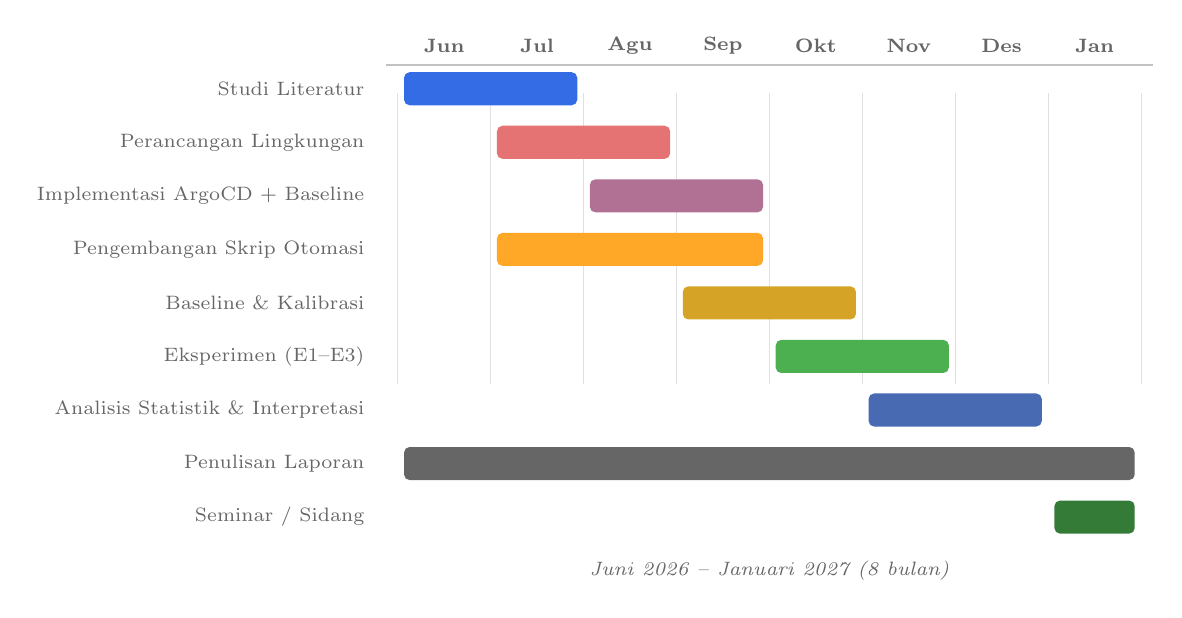
\begin{tikzpicture}[
    monthlabel/.style={font=\scriptsize\bfseries, text=manualgray},
    actlabel/.style={font=\scriptsize, align=right, text=manualgray, anchor=east},
    bar/.style={rectangle, rounded corners=2pt, fill=#1,
                 minimum height=0.42cm, inner sep=0pt},
    gridline/.style={manualgray!20, line width=0.3pt}
]

\def\colw{1.18}
\def\labelx{3.4}
\def\startx{3.7}

\foreach \i/\m in {0/Jun, 1/Jul, 2/Agu, 3/Sep, 4/Okt, 5/Nov, 6/Des, 7/Jan} {
    \node[monthlabel] at (\startx + \i*\colw + 0.5*\colw, 0.55) {\m};
}

\draw[manualgray!40, line width=0.5pt] (\startx - 0.15, 0.30) -- (\startx + 8*\colw + 0.15, 0.30);

\foreach \i in {0,...,8} {
    \draw[gridline] (\startx + \i*\colw, -0.05) -- (\startx + \i*\colw, -3.75);
}

\def\y{0.0}
\def\dy{-0.68}

\node[actlabel] at (\labelx, \y) {Studi Literatur};
\fill[bar=gitopsblue] (\startx + 0*\colw + 0.08, \y - 0.21) rectangle (\startx + 2*\colw - 0.08, \y + 0.21);

\node[actlabel] at (\labelx, \y+\dy) {Perancangan Lingkungan};
\fill[bar=driftred] (\startx + 1*\colw + 0.08, \y+\dy - 0.21) rectangle (\startx + 3*\colw - 0.08, \y+\dy + 0.21);

\node[actlabel] at (\labelx, \y+2*\dy) {Implementasi ArgoCD + Baseline};
\fill[bar=driftred!70!gitopsblue] (\startx + 2*\colw + 0.08, \y+2*\dy - 0.21) rectangle (\startx + 4*\colw - 0.08, \y+2*\dy + 0.21);

\node[actlabel] at (\labelx, \y+3*\dy) {Pengembangan Skrip Otomasi};
\fill[bar=warnorange] (\startx + 1*\colw + 0.08, \y+3*\dy - 0.21) rectangle (\startx + 4*\colw - 0.08, \y+3*\dy + 0.21);

\node[actlabel] at (\labelx, \y+4*\dy) {Baseline \& Kalibrasi};
\fill[bar=metricyellow!85!black] (\startx + 3*\colw + 0.08, \y+4*\dy - 0.21) rectangle (\startx + 5*\colw - 0.08, \y+4*\dy + 0.21);

\node[actlabel] at (\labelx, \y+5*\dy) {Eksperimen (E1--E3)};
\fill[bar=okgreen] (\startx + 4*\colw + 0.08, \y+5*\dy - 0.21) rectangle (\startx + 6*\colw - 0.08, \y+5*\dy + 0.21);

\node[actlabel] at (\labelx, \y+6*\dy) {Analisis Statistik \& Interpretasi};
\fill[bar=gitopsblue!60!manualgray] (\startx + 5*\colw + 0.08, \y+6*\dy - 0.21) rectangle (\startx + 7*\colw - 0.08, \y+6*\dy + 0.21);

\node[actlabel] at (\labelx, \y+7*\dy) {Penulisan Laporan};
\fill[bar=manualgray] (\startx + 0*\colw + 0.08, \y+7*\dy - 0.21) rectangle (\startx + 8*\colw - 0.08, \y+7*\dy + 0.21);

\node[actlabel] at (\labelx, \y+8*\dy) {Seminar / Sidang};
\fill[bar=okgreen!70!black] (\startx + 7*\colw + 0.08, \y+8*\dy - 0.21) rectangle (\startx + 8*\colw - 0.08, \y+8*\dy + 0.21);

\node[font=\scriptsize\itshape, text=manualgray, align=center] at (\startx + 4*\colw, \y+9*\dy) {Juni 2026 -- Januari 2027 (8 bulan)};

\end{tikzpicture}
\end{document}